\documentclass[11pt]{article}
\usepackage[margin=1in]{geometry}
\usepackage{graphicx}
\usepackage{booktabs}
\usepackage{hyperref}
\usepackage{amsmath}
\usepackage{enumitem}
\usepackage{xcolor}
\title{Harness Developing Agent (HDA): Phase-1 Methods and Run Report}
\author{CS 5624 project --- agent-generated draft}
\date{2026-11-21}

\begin{document}
\maketitle

\begin{abstract}
This report covers only the new Harness Developing Agent (HDA) work. It
describes the method in enough detail to be reproduced, then reports the runs
that have completed: pipeline verification, the human C++ reference, the
identifiability analysis, and a reduced Qwen3-4B pilot. The full BF16
$k=10$ grid is queued but had not started when this report was written.
\end{abstract}

\section{Scope and status}

The HDA replaces the previous \emph{library-assisted} setting, in which the
agent answers one graph instance by calling NetworkX. Here the agent writes one
self-contained C++17 program per task and the program is evaluated on graphs up
to 100{,}000 nodes. The previous Python/NetworkX results are not repeated in
this report.

Completed: the tested pipeline was installed on ARC; all 18 unit tests pass;
the data were generated; the human C++ reference and the identifiability
analysis were run; a reduced Qwen3-4B pilot and a hidden-condition smoke test
were executed.

Not completed: the intended BF16 $k=10$ grid and the BF16 smoke test. Both are
queued (Slurm 1550735 and 1550755) but were blocked by GPU reservations and
fairshare. No result in this report uses those jobs.

\section{What the HDA is}

A Harness Developing Agent is an LLM that writes a \emph{program} instead of
answering one instance. For a fixed graph task it receives $k$ input/output
examples and must produce a single C++17 file that reads any graph from stdin
and prints the answer. The file is compiled and run in a resource-limited
sandbox. The agent may test, run and stress its program, revise it, and submit
it once per iteration. The best validation submission $H^*$ is the harness that
is finally tested on held-out graphs.

This directly tests \emph{learn small, run big}: a program that is correct but
has the wrong complexity passes validation on 4--50-node graphs and fails on
large graphs.

\section{Agent interface}

\subsection{What the model sees}

\begin{table}[h]
\centering
\small
\begin{tabular}{p{3.1cm}p{10.3cm}}
\toprule
Part & Content \\
\midrule
System prompt & Role; C++17 and the standard library only (no Boost, no graph
libraries, no file I/O, threads or system calls); hidden graphs up to $1000\times$
larger with permuted node IDs; explicit ban on memorizing or hardcoding
answers, node IDs, edge lists, sizes or lookup tables; limits 1--5\,s CPU,
1\,GiB memory, 8\,MiB stack; input format; graph-loading template; tool
protocol. \\
Problem statement & \emph{Given}: one paragraph. \emph{Hidden}: no statement;
the model must list at least three candidate problems, argue for and against
each against every example, keep the simplest consistent one in
\texttt{<statement>}, and may revise it later. \\
Examples & $k=10$ new examples per iteration, drawn without replacement from
the \texttt{examples} pool (4--50 nodes, seen families). The prompt shows the
current 10; the \texttt{test} tool runs every example seen so far. \\
Iteration context & Iteration number, aggregate validation feedback from the
last submission, the best program so far with its validation accuracy, and the
current statement. \\
Tools & One action per reply: \texttt{test} (compile and run all seen examples),
\texttt{run} (custom input), \texttt{stress} (compile a C++ generator and run
the program on its output, up to 64\,MiB), \texttt{submit}. \\
Output & One C++17 source file per iteration plus the current
\texttt{<statement>}. $H^*$ is the best-validation submission; ties go to the
later iteration. \\
\bottomrule
\end{tabular}
\caption{HDA input, tools and output.}
\end{table}

\subsection{Input format}

Every graph, example or test, uses the same three-part format:
\begin{verbatim}
n m directed weighted        # directed, weighted in {0,1}
u v [w]                      # m lines, nodes 0..n-1, no self-loops
k q1 ... qk                  # query arguments (k = 0 or 2)
\end{verbatim}
The header exposes whether the graph is directed or weighted and how many query
nodes follow. This narrows the task family but does not identify the task.

Even in the hidden condition the model therefore knows the input signature.
Identification must come from the examples (Section~\ref{sec:ident}).

\section{Tasks}

Phase~1 uses ten polynomial-time tasks with exact, single-token answers:
shortest path (weighted $s$--$t$ distance), reachability (directed YES/NO),
connected-component count, cycle detection (YES/NO), diameter (connected,
unweighted), common-neighbor count, triangle count, bipartite check (YES/NO),
MST weight and max-flow value. NP-hard tasks are phase~2.

\begin{table}[h]
\centering
\small
\begin{tabular}{llllp{6.2cm}}
\toprule
task & directed & weighted & query args & statement \\
\midrule
shortest\_path & no & yes & 2 (s,t) & Given an undirected graph with positive integer edge weights and two nodes s and t (the query 2 s t), print the total weight of a minimum-weight path from s to t, or -1 if t is unreachable from s. \\
reachability & yes & no & 2 (s,t) & Given a directed graph and two nodes s and t (query 2 s t), print YES if there is a directed path from s to t, otherwise NO. \\
connected\_components & no & no & none & Given an undirected graph, print the number of connected components (an isolated node is its own component). \\
cycle\_detection & no & no & none & Given an undirected simple graph, print YES if it contains at least one cycle, otherwise NO. \\
diameter & no & no & none & Given a connected undirected unweighted graph, print its diameter: the largest shortest-path distance (in edges) between any two nodes. \\
common\_neighbors & no & no & 2 (s,t) & Given an undirected graph and two nodes u and v (query 2 u v), print the number of nodes adjacent to both u and v. \\
triangle\_count & no & no & none & Given an undirected simple graph, print the number of triangles (unordered triples of mutually adjacent nodes). \\
bipartite\_check & no & no & none & Given an undirected graph, print YES if its nodes can be split into two sets so that every edge joins the two sets (the graph is bipartite), otherwise NO. \\
mst\_weight & no & yes & none & Given a connected undirected graph with positive integer edge weights, print the total weight of a minimum spanning tree. \\
max\_flow & yes & yes & 2 (s,t) & Given a directed graph whose edge weights are capacities and two nodes s and t (query 2 s t), print the value of a maximum flow from s to t. \\
\bottomrule
\end{tabular}

\caption{Phase-1 tasks.}
\end{table}

\section{Data generator and splits}

\subsection{Families and shaping}

Seen families (examples and validation): Erd\H{o}s--R\'enyi,
Barab\'asi--Albert, random trees (bushy and path-like), and disjoint unions.
Unseen families (test only): Watts--Strogatz, 2-D grids with 10\% of edges
removed, caterpillar/path-like graphs, dense ER ($p=0.3$--$0.6$,
$n\le1000$), random regular, and powerlaw-cluster.

Average degree cycles through 1.2--3, 3--8 and 8--20. Tasks are shaped so the
answer is not degenerate: diameter and MST graphs are connected; cycle
detection is balanced between forests and forests plus 1--3 chords; bipartite
is balanced between bipartite and one-odd-edge graphs; reachability queries are
50/50; shortest-path and max-flow are 85\% reachable; common-neighbor queries
use a 2-hop pair 70\% of the time. Directed graphs keep about 25\% of edges in
both directions. Weights are 1--100, capacities 1--50.

Node IDs are randomly permuted and edge and endpoint order are shuffled. This
is the first anti-shortcut layer: a program cannot rely on node labels or edge
position.

\subsection{Splits}

\begin{table}[h]
\centering
\small
\begin{tabular}{llrrlr}
\toprule
split & nodes & n/task & fam. & limit (s) \\
\midrule
examples & 4-50 & 120 & seen & 1 \\
val & 4-50 & 40 & seen & 1 \\
test\_small & 4-50 & 40 & all & 1 \\
test\_medium & 100-300 & 30 & all & 2 \\
test\_large & 500-1000 & 30 & all & 2 \\
test\_xl & 2000-2000 & 20 & all & 3 \\
test\_stress & 10000-100000 & 10 & all & 5 \\
\bottomrule
\end{tabular}

\caption{Splits, node ranges, per-task counts, families and CPU limits.}
\end{table}

Base seed 5625; each split uses a different seed offset, so no graph is shared.
The HDA sees only the 10 examples of the current iteration; validation and test
graphs are never shown. The \texttt{examples} pool has 120 graphs per task, so
five iterations use 50 of them and the remaining 70 are unused.

\subsection{Ground truth}

Ground truth comes from human-written C++ reference solvers in
\texttt{reference/*.cpp}. They are cross-checked against NetworkX on 600 random
graphs by the test suite, and are also run through the same sandbox as the HDA
programs to measure the human upper bound.

\section{Training loop}

One run is a triple (task, condition, seed). It executes the following loop:

\begin{enumerate}[leftmargin=1.4em]
\item For iteration $t=1,\dots,5$, draw 10 new examples from the pool and show
them with the last validation feedback, the best program so far and the current
statement.
\item The HDA works for at most 8 tool steps. Each reply is parsed for one
action, the latest \texttt{cpp} block and the current \texttt{<statement>}.
\item On \texttt{submit} (or when the step budget ends), the latest program is
checked by the static policy. A violation gives score 0 and the reason is
returned as feedback.
\item The program is compiled. A compile error also gives score 0 and the
compiler output is returned.
\item The program is scored on 40 hidden validation graphs (4--50 nodes, seen
families). Five validation graphs are re-run with fresh node IDs; each
relabeling failure reduces the iteration score proportionally.
\item Feedback contains accuracy, verdict counts (AC/WA/TLE/RE/MLE), accuracy
by size bucket and family, and the maximum CPU time.
\end{enumerate}

After five iterations, $H^*$ is the submission with the best validation
accuracy. It is evaluated once on \texttt{test\_small}, \texttt{test\_medium},
\texttt{test\_large}, \texttt{test\_xl} and \texttt{test\_stress}. The problem
statement is logged at every step but is not scored during training.


\section{Training and validation loop: components and I/O}
\label{sec:loop-diagram}

Figure~\ref{fig:loop} shows one run. The inner loop is the \emph{step loop}
(at most 8 replies); the outer loop is the \emph{iteration loop} (at most 25
iterations in the current shortest-path run, 5 in the standard grid). Only the
C++ block is compiled and scored; the statement and reasoning are logged but
never passed to the evaluator.

\begin{figure}[p]
\centering
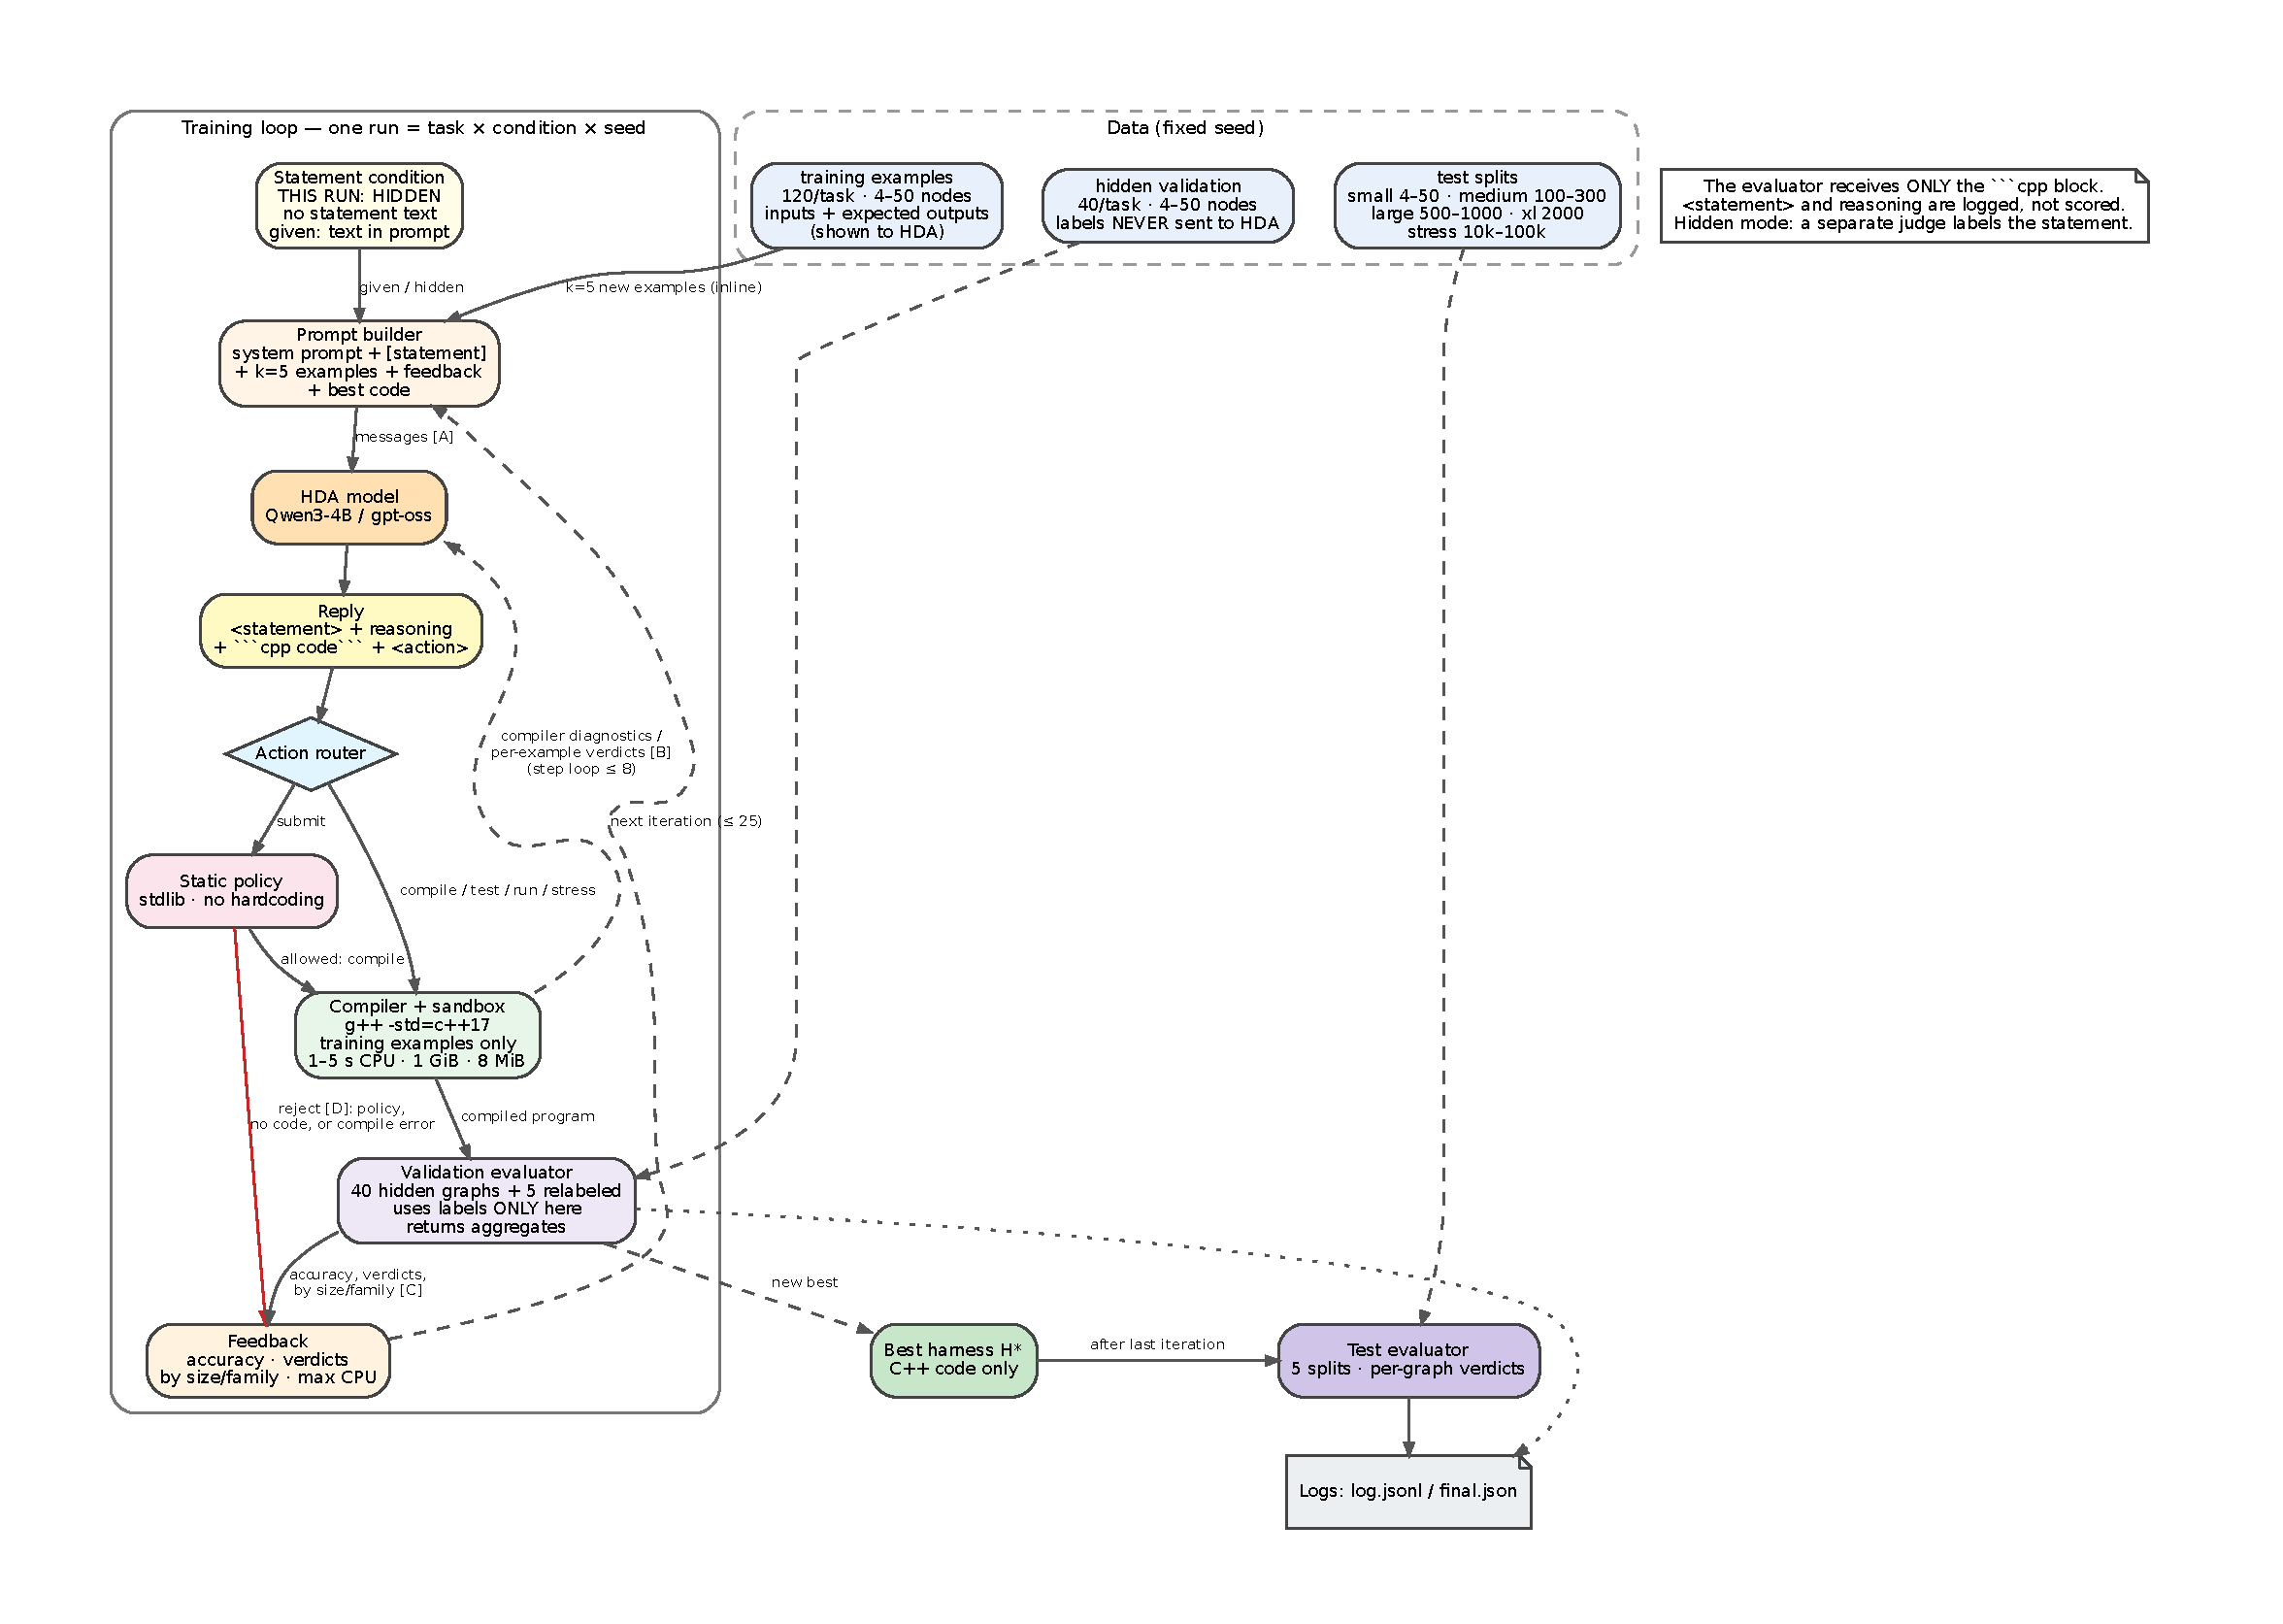
\includegraphics[width=0.95\linewidth]{figures/hda/hda_loop.pdf}
\caption{Training and validation loop. Solid arrows are data flow, dashed
arrows are feedback or control. The evaluator receives only the \texttt{cpp}
block.}
\label{fig:loop}
\end{figure}

\begin{table}[p]
\centering
\small
\begin{tabular}{p{3.0cm}p{4.6cm}p{5.6cm}}
\toprule
Component & Input & Output \\
\midrule
Data generator & split config (seed, node range, per-task count,
families) & JSONL graph records with input text and expected answer; C++
reference answers \\
Prompt builder & system prompt, given/hidden condition, the $k$ new examples,
last feedback, best code, iteration index & one message list (system + user)
for the model \\
HDA model & message list & reply containing \texttt{<statement>}, optional
reasoning, a \texttt{cpp} block, and one action tag \\
Action router & reply & tool call (\texttt{compile}, \texttt{test},
\texttt{run}, \texttt{stress}) or \texttt{submit}; no code on submit is
rejected \\
Compiler + sandbox & C++ source, stdin, limits (1--5\,s, 1\,GiB, 8\,MiB
stack) & compiler diagnostics; stdout/stderr; verdict AC/WA/TLE/RE/MLE; CPU
seconds \\
Static policy & C++ source, example answers & allow/reject with a reason
(headers, I/O, threads, hardcoded tables) \\
Validation evaluator & compiled program, 40 hidden validation graphs, 5
relabeled copies & accuracy, verdict mix, accuracy by size and family, max
CPU, relabeling failures \\
Feedback builder & validation summary, policy/compile result & short text
returned to the prompt builder \\
Best-harness tracker & per-iteration code and validation score & $H^*$ (the
best C++ program); ties go to the later iteration \\
Test evaluator & $H^*$, the five test splits & per-graph verdicts and
per-split accuracy; no test graph is shown to the HDA \\
Statement judge (hidden) & true statement, inferred statement & EQUIVALENT /
PARTIAL / WRONG; not used for scoring the program \\
Logger & every event above & \texttt{log.jsonl} (prompts, replies, tools,
submissions, iterations, tests) and \texttt{final.json} \\
\bottomrule
\end{tabular}
\caption{Components, inputs and outputs.}
\label{tab:components}
\end{table}

\section{Given and hidden problem statements}
\label{sec:ident}

In the \emph{given} condition the model sees the task statement. In the
\emph{hidden} condition it must infer the task from the examples, write a
candidate statement in \texttt{<statement>}, and may revise it later. We record
the statement at every step; an LLM judge labels the final statement
EQUIVALENT/PARTIAL/WRONG, and functional identification is test-small accuracy
$\ge95\%$.

The pipeline measures how many candidate tasks remain consistent with $k$
examples. Candidates are the 10 tasks plus 37 distractors (edge count, maximum
degree, connectivity, triangle existence, edge weight, strong connectivity,
widest path, out-capacity of $s$, and so on). Table~\ref{tab:ident} reports the
probability that the true task is the unique survivor over 400 trials.

\begin{table}[h]
\centering
\small
\begin{tabular}{lrrrrrp{4.5cm}}
\toprule
task & candidates & k=1 & k=3 & k=5 & k=10 & top confusers at k=3 \\
\midrule
shortest\_path & 4 & 0.81 & 0.98 & 1.00 & 1.00 & edge\_weight, max\_edge\_on\_path \\
reachability & 5 & 0.00 & 0.18 & 0.45 & 0.86 & strongly\_connected, edge\_exists, undirected\_connected \\
connected\_components & 18 & 0.76 & 1.00 & 1.00 & 1.00 & radius\_lcc \\
cycle\_detection & 18 & 0.01 & 0.41 & 0.67 & 0.93 & has\_triangle, is\_connected, is\_tree \\
diameter & 18 & 0.78 & 1.00 & 1.00 & 1.00 & -- \\
common\_neighbors & 7 & 0.60 & 0.97 & 1.00 & 1.00 & min\_degree\_uv, degree\_v, degree\_u \\
triangle\_count & 18 & 0.43 & 0.90 & 0.97 & 1.00 & cycle\_rank, isolated\_nodes \\
bipartite\_check & 18 & 0.23 & 0.74 & 0.92 & 1.00 & is\_connected, is\_tree, cycle\_detection \\
mst\_weight & 6 & 0.58 & 0.93 & 0.98 & 1.00 & max\_spanning\_tree, total\_weight \\
max\_flow & 7 & 0.16 & 0.54 & 0.77 & 0.98 & min\_out\_in, widest\_path, out\_capacity\_s \\
\bottomrule
\end{tabular}

\caption{Probability that the true task is the unique survivor among 10 tasks
and 37 distractors, and the main confusers at $k=3$ (400 trials).}
\label{tab:ident}
\end{table}

At $k=10$, every task is identifiable in at least 86\% of draws. Reachability
(0.86) and cycle detection (0.93) are the hardest; later iterations add ten more
examples. This supports the fixed choice $k=10$.

\section{Anti-memorization}

Four layers are active:

\begin{enumerate}[leftmargin=1.4em]
\item \textbf{Prompt.} The system prompt forbids memorizing or hardcoding
answers, node IDs, edge lists, sizes, lookup tables or special cases, and says
such programs are rejected and relabeling-checked.
\item \textbf{Static policy.} Only standard headers are allowed; system calls,
file I/O, threads/OpenMP, inline assembly and local includes are banned. The
policy also rejects literal arrays of 20+ numbers, more than 24 non-trivial
numeric literals, and code containing two or more example answers verbatim.
\item \textbf{Behavioral.} Validation and test graphs are fresh and hidden; node
IDs are permuted; five graphs per evaluation are re-run with new node IDs and
must give the same answer.
\item \textbf{Sandbox.} An empty working directory, input on stdin only, and
CPU/memory/stack/output limits prevent a program from reading test files.
\end{enumerate}

\section{Evaluation and logging}

Metrics are accuracy, verdict mix, the small--large gap
(\texttt{test\_small} minus \texttt{test\_xl}), accuracy by size, family and
density, identification and cost (tokens, wall time, tool calls). Baselines are
a one-shot HDA (1 iteration), the majority answer, the human C++ reference and
the older library-assisted Python/NetworkX harness.

Each run writes \texttt{log.jsonl}, one JSON event per line:
\texttt{config}, \texttt{examples}, \texttt{prompt}, \texttt{reply} (raw text,
reasoning trace when the server returns one, action, statement, code, token
counts), \texttt{tool}, \texttt{submission} (policy, code, answers on every
example and validation graph), \texttt{iteration}, \texttt{judge} and
\texttt{test}. \texttt{final.json} contains the validation curve, statements,
judge label, tokens and test summaries. Logs stay out of git; \texttt{final.json}
and the best program are committed.

\section{Runs performed}

\subsection{H0: installation and verification (CPU)}

On ARC, with Python 3.13.11, NetworkX 3.7, g++ 11.5 and C++17:

\begin{verbatim}
python -m pytest -q tests
python -m hda.generator --out data/hda
python -m hda.human_baseline --out experiments/hda/human_reference
python -m hda.identifiability --data data/hda --trials 400 \
       --out experiments/hda/identifiability.json
\end{verbatim}

Results:

\begin{itemize}[leftmargin=1.4em]
\item 18/18 tests pass (reference vs NetworkX, balance, verdicts, stack
overflow, policy, scripted agent loop, stress tool).
\item Data build: 60\,s. examples 1{,}200; val 400; test\_small 400;
test\_medium 300; test\_large 300; test\_xl 200; test\_stress 100.
\item Human reference: 100\% on every task and split. Maximum CPU time:
0.0065\,s (val), 0.0061\,s (small), 0.0115\,s (medium), 0.2263\,s (large),
0.0888\,s (xl), 0.4482\,s (stress), all below one third of the limits.
\item Identifiability: see Table~\ref{tab:ident}.
\end{itemize}

\subsection{Qwen3-4B reduced pilot (Q4 CPU)}

Because gpt-oss-120b is not on disk and all B200 GPUs were reserved, the only
model run is a deliberately reduced diagnostic: Qwen3-4B-Instruct-2507
(Q4\_K\_M, llama.cpp CPU server, 8{,}192-token context, 32 threads), given
condition, $k=3$, one iteration, four tool steps, 2{,}048 maximum tokens,
tested on \texttt{test\_small}. Nine of the ten tasks completed; cycle
detection exceeded the 8k context (9{,}023 prompt + 2{,}048 completion tokens)
and produced no result.

\begin{table}[h]
\centering
\small
\begin{tabular}{lrrrrrr}
\toprule
task & condition & k & iters & best val & test\_small & judge \\
\midrule
bipartite\_check & given & 3 & 1 & 44.0\% & 52.5\% &  \\
common\_neighbors & given & 3 & 1 & 11.0\% & 20.0\% &  \\
connected\_components & given & 3 & 1 & 0.0\% & -- &  \\
diameter & given & 3 & 1 & 0.0\% & -- &  \\
max\_flow & given & 3 & 1 & 0.0\% & -- &  \\
mst\_weight & given & 3 & 1 & 100.0\% & 100.0\% &  \\
reachability & given & 3 & 1 & 0.0\% & -- &  \\
shortest\_path & given & 3 & 1 & 0.0\% & -- &  \\
triangle\_count & given & 3 & 1 & 0.0\% & -- &  \\
\bottomrule
\end{tabular}

\caption{Reduced Qwen3-4B pilot (Q4 CPU, $k=3$, one iteration, four steps).
Cycle detection is absent because it exceeded the 8k context. ``--'' means the
submission did not compile, so no test was run.}
\end{table}

Interpretation of the pilot:

\begin{itemize}[leftmargin=1.4em]
\item MST weight and bipartite check produce working programs and non-zero
test accuracy (100\% and 52.5\%). Common neighbors reaches 20\% on test.
\item The six zero tasks mostly fail at compile time because the model's code
block omits the provided loader/template and refers to an undefined graph
object. A few are policy/parse failures.
\item Hidden-condition smoke (diameter, $k=3$, three steps): the model spent
every step debating candidate statements and submitted no code, so score 0.
\item This is a model-strength result, not a pipeline failure: the same
pipeline's human references score 100\% and all component tests pass.
\end{itemize}

\subsection{Queued but not run}

\begin{itemize}[leftmargin=1.4em]
\item Slurm 1550735: Qwen3-4B BF16, 32k context, $k=10$, 5 iterations,
8 steps, 10 tasks $\times$ 2 conditions $\times$ 3 seeds (60 runs), projected
start 19:10.
\item Slurm 1550755: the same model, $k=10$ diameter given smoke, projected
00:46.
\end{itemize}

No numbers from these jobs are included.

\section{Discussion}

The completed work validates the infrastructure and the experimental design:
data generation, human upper bound, identifiability, policy, sandbox, logging
and scoring all behave as specified. The reduced Qwen pilot shows that a 4B
model can occasionally produce a correct standalone solver (MST, bipartite) but
usually fails to emit a complete C++ file or gets stuck on the hidden-statement
inference, which is consistent with the earlier C-backend pilot (12\% on small
graphs).

The main scientific question---whether a strong HDA learns small and runs
big---cannot be answered from this pilot. It requires the BF16 $k=10$ grid, and
ideally the hidden condition with enough tokens for statement inference.

\section{Limitations}

\begin{itemize}[leftmargin=1.4em]
\item The only model result is Qwen3-4B Q4 on CPU, $k=3$, one iteration; it is
not comparable to the intended gpt-oss-120b/BF16 setting.
\item The header reveals directed/weighted and the number of query nodes, so
the hidden task is only partially hidden.
\item The judge is the same model family as the HDA, and was not exercised on
the completed pilot (hidden smoke produced no statement).
\item gpt-oss-120b is not on disk; downloading it (~65\,GB) and the BF16 grid
remain pending.
\item All HDA prose in the course report is an AI draft and must be rewritten
by the authors.
\end{itemize}

\section{Reproduction}

\begin{verbatim}
cd hda_pipeline
python -m pytest -q tests
python -m hda.generator --out data/hda
python -m hda.human_baseline --out ../experiments/hda/human_reference
python -m hda.identifiability --data data/hda --trials 400 \
       --out ../experiments/hda/identifiability.json
python -m hda.agent --task mst_weight --condition given --k 3 --n-iter 1 \
       --steps 4 --out ../experiments/hda/qwen_cpu_pilot2/mst_weight/given \
       --model qwen3-4b-q4 --base-url http://127.0.0.1:8002/v1 \
       --max-tokens 2048 --reasoning-effort "" --test-splits test_small
\end{verbatim}

Artifacts: \texttt{experiments/hda/human\_reference/},
\texttt{experiments/hda/identifiability.json},
\texttt{experiments/hda/qwen\_cpu\_pilot2/},
\texttt{experiments/hda/smoke\_qwen\_cpu/},
\texttt{report/tables/hda/}.

\end{document}
